\section{Measurement Procedure} \label{sec:results:procedure}

To measure the Standard Model signal of interest a model comprised of $V$ +
jets, $H \rightarrow b\bar{b}$ and $t\bar{t}$ templates along with a QCD
multijet model is is fit to the data. The $t\bar{t}$ template is constructed
from a MC sample with its normalization corrected with a $k$-factor derived
from a dedicated $t\bar{t}$ Control Region. This fit simultaneously extracts
the signal strengths of the $V$ + jets and $H \rightarrow b\bar{b}$ process,
$\mu_{V}$ and $\mu_{H}$ respectively, which are parameterized with a flat
prior. The comparison of data to the maximum a posterior probability (post-fit)
model is seen in \Cref{sec:results:money_plot}.

\begin{figure}
\centering
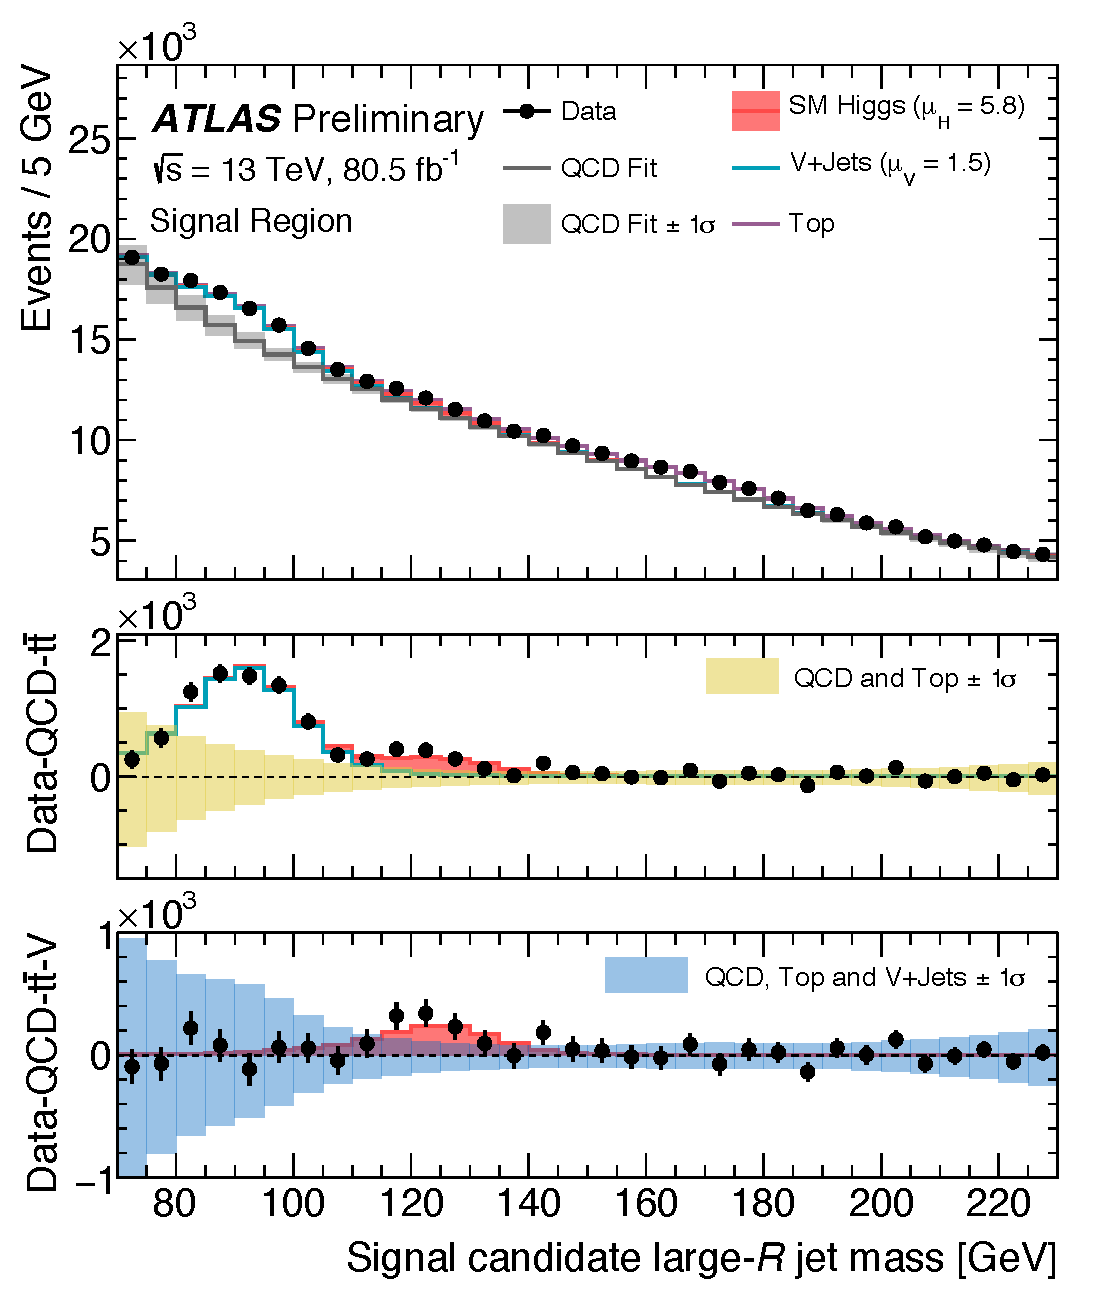
\includegraphics[width=\linewidth]{figures/results/money_plot}
\caption{\cite{ATLAS-CONF-2018-052} 
The top panel shows the post-fit comparison of the signal candidate large-$R$
jet mass distribution for the combined SM Higgs boson, $V$ + jets, $t\bar{t}$
and QCD model to the observed data.  The middle panel gives the ratio of the
post-fit model and the data with the QCD and $t\bar{t}$ components subtracted,
highlighting the large resonance from $V$ + jets.  The bottom panel gives the
ratio of the post-fit model and the data with the QCD, $V$ + jets, and
$t\bar{t}$ components subtracted, highlighting a slight excess of events near
$m_{J} = 125~\GeV$}
\label{sec:results:money_plot}
\end{figure}

